
          %------------------------%
\chapter{~~Cells, meshes, iterators}\label{\numb section 9}
          %------------------------%


This section gives details about cells and meshes.

          %-------------------------%
\section{~~Building cells and meshes}\label{\numb section 9.\numb parag 1}
          %-------------------------%

As we have already seen in examples in sections \ref{\numb section 2} and \ref{\numb section 3},
cells and meshes are created by declaring them as {\small\tt \verm{Cell}} or
{\small\tt \verm{Mesh}} objects
and by providing specific options to their constructor, by means of {\small\tt\textcolor{tag}{tag}}s.
For instance :

\begin{Verbatim}[commandchars=\\\{\},formatcom=\small\tt,
   baselinestretch=0.94,framesep=2mm                      ]
   \verm{Cell} \azul{SW} ( \textcolor{tag}{tag}::vertex ); \cinza{// and the same for vertices SE, NE, NW}
   \verm{Mesh} \azul{south} ( \textcolor{tag}{tag}::segment, SW .reverse(), SE, \textcolor{tag}{tag}::divided_in, \laranja{10} );
   \cinza{// similar declarations of east, north, west}
   \verm{Mesh} \azul{rectangle} ( \textcolor{tag}{tag}::rectangle, south, east, north, west );
\end{Verbatim}

Paragraph \ref{\numb section 11.\numb parag 3} gives more details about {\small\tt\textcolor{tag}{tag}}s.

Internally, {\maniFEM} implements cells and meshes as persistent objects, built
using the {\small\tt new} operator and thus having no syntactic scope.
Objects belonging to classes {\small\tt \verm{Cell}} and {\small\tt \verm{Mesh}} are just a wrapper
around a persistent core (cell or mesh).
When they go out of scope, the wrappers are destroyed; the core may remain alive or not,
depending on its relationships with other cells and meshes.
This is explained in paragraph \ref{\numb section 11.\numb parag 5}.

Cells and meshes are unique objects, it makes no sense to copy them.
A statement like {\small\tt \verm{Cell}} {\small\tt copy\_\,of\_\,A} {\small\tt =} {\small\tt A}
will make a copy of the wrapper but it will refer to the same cell {\small\tt A}.
If you change e.g.\ a coordinate of {\small\tt copy\_\,of\_\,A}, the coordinate of {\small\tt A}
will also change.
That is, wrapper classes {\small\tt \verm{Cell}} and {\small\tt \verm{Mesh}} can be viewed as
customized pointers.
This is useful if we need to create many meshes in a loop, as shown in paragraph
\ref{\numb section 9.\numb parag 2}.
However, there are operations which do create a new cell or mesh.
There are also operations which create a new cell or mesh only if necessary,
otherwise they will return an existing cell or mesh.
Paragraph \ref{\numb section 9.\numb parag 10} gives a complete list.

Recall that, in \maniFEM, cells and meshes are oriented.
When a cell is declared, it is built as positive and has no reverse.
Its reverse is a negative cell and will be built only if necessary.
Cells have a method {\small\tt reverse} which does the following.
It checks if the reverse object has already been built; if yes, it returns that object;
otherwise, it builds the reverse cell on-the-fly and returns it.
Paragraph \ref{\numb section 9.\numb parag 5} gives a more detailed explanation about
orientation of cells and meshes.
% See also paragraph \ref{\numb section 11.\numb parag 4}.

{\small\tt \verm{Mesh}}es have also a {\small\tt reverse} method.
Note that reverse meshes exist always (negative meshes are temporary objects built
on-the-fly).

At a basic level, the only situation when you need the {\small\tt reverse} method  for cells is
when you declare a segment {\small\tt \verm{Mesh}} (you must provide a negative
{\small\tt \verm{Cell}} as starting point).
You will occasionaly need to use the {\small\tt reverse} method for meshes (for instance, if you
intend to {\small\tt join} two meshes, their common boundary must have a certain orientation when
seen from a mesh and the opposite orientation when seen from the other mesh).
In the example in paragraph \ref{\numb section 1.\numb parag 4},
reverses of meshes {\small\tt CD} and {\small\tt BC} are used.


          %------------------%
\section{~~A ring-shaped mesh}\label{\numb section 9.\numb parag 2}
          %------------------%

For creating many meshes within a cycle, we can view a {\small\tt \verm{Cell}} object as a
(customized) pointer to a persistent core cell, and the same for {\small\tt \verm{Mesh}}es.
They are cheap to store and to copy.
We call these customized pointers ``wrappers''; their behaviour is described in some detail in
paragraph \ref{\numb section 11.\numb parag 4}.

\begin{figure}[ht] \centering
  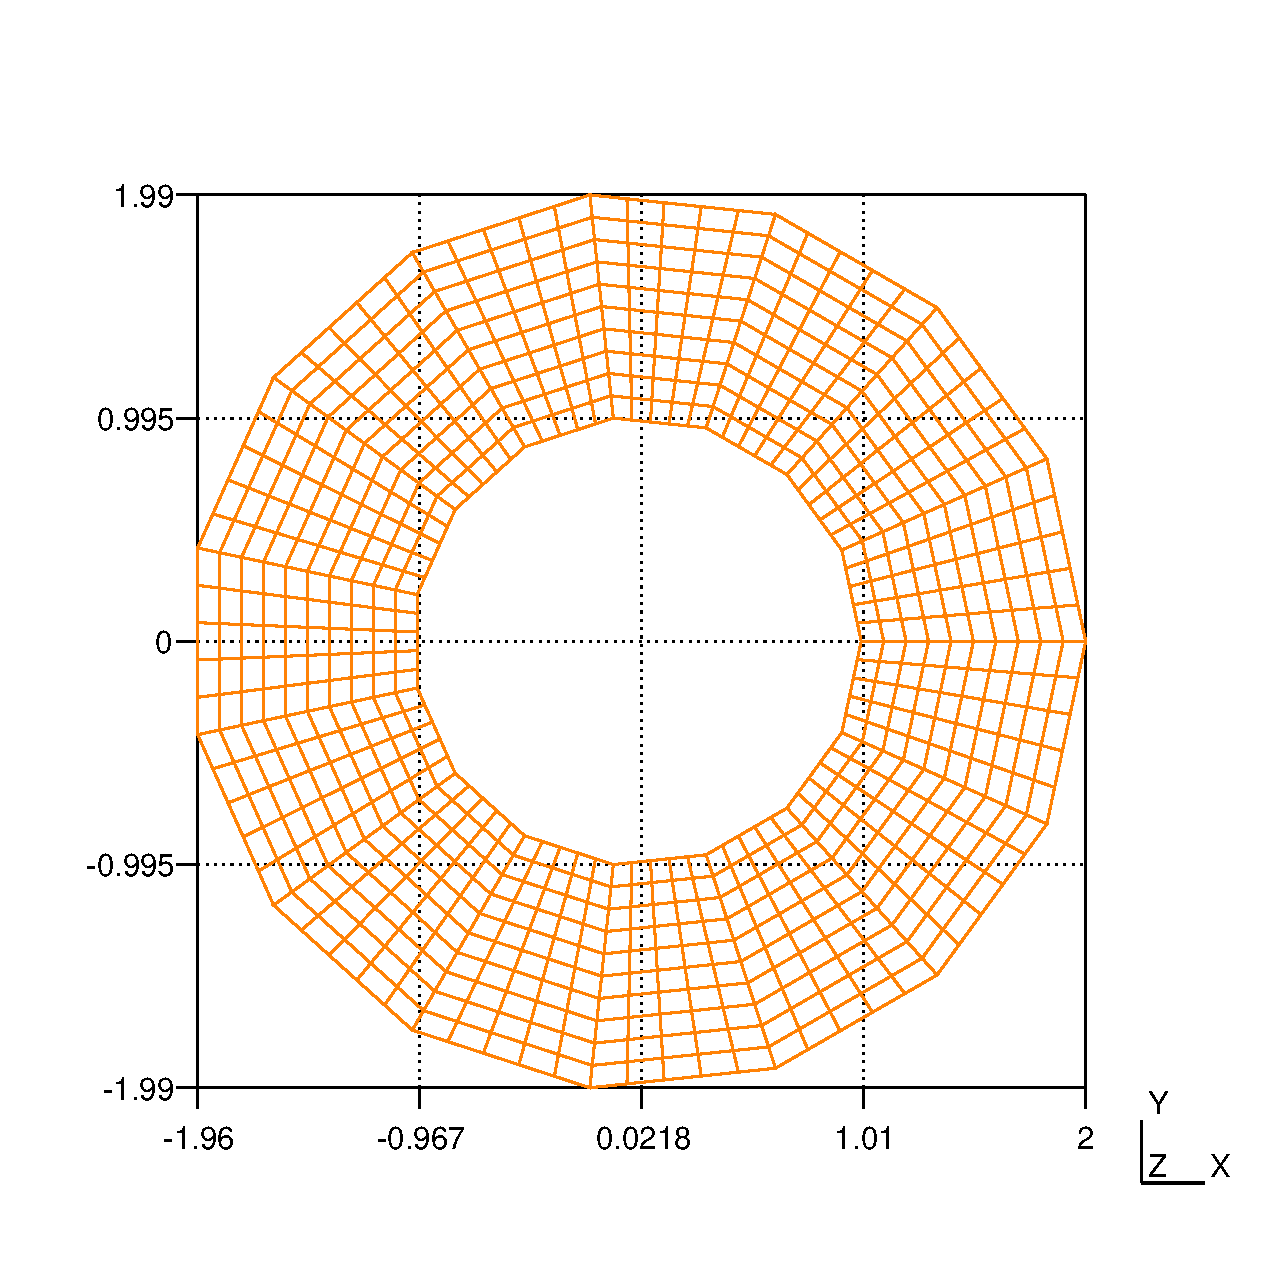
\includegraphics[width=115mm]{ring.eps}
  \caption{A ring-shaped mesh}
  \label{\numb section 9.\numb fig 1}
\end{figure}

\begin{Verbatim}[commandchars=\\\{\},formatcom=\small\tt,frame=single,
   label=parag-\ref{\numb section 9.\numb parag 2}.cpp,rulecolor=\color{coment},
   baselinestretch=0.94,framesep=2mm                                            ]
   \verm{FManifold} \azul{RR2} ( \textcolor{tag}{tag}::Euclid, \textcolor{tag}{tag}::of_dim, \laranja{2} );
   \verm{Function} \azul{xy} = RR2 .build_coordinate_system ( \textcolor{tag}{tag}::Lagrange, \textcolor{tag}{tag}::of_degree, \laranja{1} );
   \verm{Function} \azul{x} = xy [\laranja{0}], \azul{y} = xy [\laranja{1}];

   short int \azul{n_sectors} = \laranja{15};
   double \azul{step_theta} = \laranja{8} * atan(\laranja{1.}) / n_sectors;
   short int \azul{radial_divisions} = \laranja{10};
   short int \azul{rot_divisions} = \laranja{5};

   \cinza{// start the process by building a segment}
   \verm{Cell} \azul{ini_A} ( \textcolor{tag}{tag}::vertex );  x ( ini_A ) = \laranja{1.};  y ( ini_A ) = \laranja{0.};
   \verm{Cell} \azul{ini_B} ( \textcolor{tag}{tag}::vertex );  x ( ini_B ) = \laranja{2.};  y ( ini_B ) = \laranja{0.};
   \verm{Mesh} \azul{ini_seg} ( \textcolor{tag}{tag}::segment, ini_A .reverse(), ini_B,
                  \textcolor{tag}{tag}::divided_in, radial_divisions     );
   \verm{Mesh} \azul{prev_seg} = ini_seg;
   \verm{Cell} \azul{A} = ini_A,  \azul{B} = ini_B;
   std::vector < \verm{Mesh} > \azul{sectors};

   for ( short int \azul{i} = \laranja{1}; i < n_sectors; i++ )
   \{  double \azul{theta} = i * step_theta;
      \cinza{// we build two new points}
      \verm{Cell} \azul{C} ( \textcolor{tag}{tag}::vertex );  x (C) = \verm{cos}(theta);     y (C) = \verm{sin}(theta);
      \verm{Cell} \azul{D} ( \textcolor{tag}{tag}::vertex );  x (D) = \laranja{2.}*\verm{cos}(theta);  y (D) = \laranja{2.}*\verm{sin}(theta);
      \cinza{// and three new segments}
      \verm{Mesh} \azul{BD} ( \textcolor{tag}{tag}::segment, B .reverse(), D, \textcolor{tag}{tag}::divided_in, rot_divisions );
      \verm{Mesh} \azul{DC} ( \textcolor{tag}{tag}::segment, D .reverse(), C, \textcolor{tag}{tag}::divided_in, radial_divisions );
      \verm{Mesh} \azul{CA} ( \textcolor{tag}{tag}::segment, C .reverse(), A, \textcolor{tag}{tag}::divided_in, rot_divisions );
      \verm{Mesh} \azul{quadr} ( \textcolor{tag}{tag}::quadrangle, prev_seg, BD, DC, CA );
      sectors .push_back ( quadr );
      prev_seg = DC .reverse();
      A = C;  B = D;                                                             \}

   \cinza{// we now build the last sector, thus closing the ring}
   \cinza{// prev_seg, A and B have rotated during the construction process}
   \cinza{// but ini_seg, ini_A and ini_B are the same, initial, ones}
   \verm{Mesh} \azul{outer} ( \textcolor{tag}{tag}::segment, B .reverse(), ini_B, \textcolor{tag}{tag}::divided_in, rot_divisions );
   \verm{Mesh} \azul{inner} ( \textcolor{tag}{tag}::segment, ini_A .reverse(), A, \textcolor{tag}{tag}::divided_in, rot_divisions );
   \verm{Mesh} \azul{quadr} ( \textcolor{tag}{tag}::quadrangle, outer, ini_seg .reverse(), inner, prev_seg );
   sectors.push_back ( quadr );
   
   \verm{Mesh} \azul{ring} ( \textcolor{tag}{tag}::join, sectors );
   ring .export_msh (\verde{"ring.msh"});
\end{Verbatim}

Note how we use a version of the {\small\tt \verm{Mesh}} constructor with {\small\tt \textcolor{tag}{tag}::join}
taking as argument a vector of {\small\tt \verm{Mesh}}es; we have already seen it in paragraphs
\ref{\numb section 2.\numb parag 7} and \ref{\numb section 2.\numb parag 11}.

We might have set curved boundaries by using a submanifold of $ \mathbb{R}^2 $, like in paragraph
\ref{\numb section 2.\numb parag 9}.

See also paragraph \ref{\numb section 11.\numb parag 8}.


          %--------------------%
\section{~~Iterators over cells}\label{\numb section 9.\numb parag 3}
          %--------------------%

As explained in paragraph \ref{\numb section 1.\numb parag 2}, a {\small\tt \verm{Mesh}} is
roughly a list of cells.
Internally, {\maniFEM} keeps lists of cells of each dimension, up the the maximum
dimension which is the dimension of the mesh.
Thus, if {\small\tt msh} is a {\small\tt \verm{Mesh}} object, modelling a
mesh of triangles, then {\small\tt msh.core->cells[0]} is a list of (wrappers) of
each vertex of that mesh, {\small\tt msh.core->cells[1]} is a list of (wrappers) of
each segment and {\small\tt msh.core->cells[2]} is a list of (wrappers) of each triangle.

Thus, if we want to iterate over all segments of a mesh, we could use an
{\small\tt std::list<\verm{Cell}>:: ::iterator}.
If you are not familiar with the notion of iterator over a list (or over other containers)
in {\tt C++}, this may be a good time for you to read an introductory book on the
{\tt C++} Standard Template Library (STL).

On the other hand, a cell is roughly defined by its boundary which in turn is a mesh of
lower dimension.
Thus, the same type of {\small\tt std::list<\verm{Cell}>::iterator} could be used to
implement a loop, say, over all vertices of a cube.

However, implementation details make this solution unpractical.
For instance, negative meshes do not keep any list,
they just hold a pointer towards their positive counterpart.
Recall that the boundary of a negative cell is a negative mesh.
Even among positive meshes, some are implemented with the goal of saving space in the
computer's memory and store less information (connected one-dimensional meshes are an
example).
Paragraph \ref{\numb section 11.\numb parag 6} describes the implementation of different
types of meshes.

For these reasons, {\maniFEM} provides objects which iterate over cells.
Suppose we have a mesh {\small\tt msh} of rectangles.
If we want to do something to each rectangle, that is, to each two-dimensional cell,
we can use a code like

\begin{Verbatim}[commandchars=\\\{\},formatcom=\small\tt,
   baselinestretch=0.94,framesep=2mm                      ]
   \verm{Mesh}::Iterator \azul{it} = msh .iterator ( \textcolor{tag}{tag}::over_cells_of_dim, \laranja{2} );
   for ( it .reset(); it .in_range(); it++ )
   \{  \verm{Cell} \azul{cll} = *it;  do_something_to (cll);  \}
\end{Verbatim}

Paragraph \ref{\numb section 11.\numb parag 3} gives some details about {\small\tt\textcolor{tag}{tag}}s.

In the above code you may note that these iterators obey to syntactic conventions
slightly different from the ones in the Standard Template Library.
We have chosen that, when we want to start an iteration process, we set the iterator in
a starting configuration by using a {\small\tt reset} method rather than through an assignment
like {\small\tt it = container.begin()}.
Similarly, when an iterator has offered access to all cells of a mesh and cannot find
other cells, it goes into a state which can be checked using its {\small\tt in\_\,range} method
rather than by testing equality with some abstract object like {\small\tt container.end()}.
We have kept the syntax {\small\tt it++} for advancing an iterator in the process of
running over cells, offering also the equivalent alteratives {\small\tt ++it} and
{\small\tt it.advance()}.
We have also kept the notation {\small\tt *it} for dereferencing a
{\small\tt \verm{Mesh}::Iterator};
this operation returns a {\small\tt \verm{Cell}} object (a wrapper).
Of course, dereferencing a {\small\tt \verm{Mesh}::Iterator} does not produce a new cell,
just provides access to a previously built cell
(with the slight exception described in paragraph \ref{\numb section 9.\numb parag 8};
see also paragraph \ref{\numb section 9.\numb parag 10}).

Often, we {\small\tt reset} an iterator only once, use it in a loop and then discard it.
For this situation, a handy shortcut is to add the {\small\tt\textcolor{tag}{tag}::reset}
to the constructor itself, as in the code excerpt below.
This has the advantage that the name of the iterator gains local scope.
(this feature is not yet implemented)

\begin{Verbatim}[commandchars=\\\{\},formatcom=\small\tt,
   baselinestretch=0.94,framesep=2mm                      ]
   for ( \verm{Mesh}::Iterator \azul{it} = msh .iterator ( \textcolor{tag}{tag}::over_cells_of_dim, \laranja{2}, \textcolor{tag}{tag}::reset );
         it .in_range(); it++                                                       )
   \{  \verm{Cell} \azul{cll} = *it;  do_something_to (cll);  \}
\end{Verbatim}

If we want to iterate over all vertices of the mesh, we can use

\begin{Verbatim}[commandchars=\\\{\},formatcom=\small\tt,
   baselinestretch=0.94,framesep=2mm                      ]
   \verm{Mesh}::Iterator \azul{it} = msh .iterator ( \textcolor{tag}{tag}::over_cells_of_dim, \laranja{0} );
   \cinza{// or, equivalently :  CellIterator it = msh .iterator ( tag::over_vertices )}
   for ( it .reset(); it .in_range(); it++ )
   \{  \verm{Cell} \azul{P} = *it;  do_something_to (P);  \}
\end{Verbatim}

If we want to iterate over all segments of the mesh, we can use

\begin{Verbatim}[commandchars=\\\{\},formatcom=\small\tt,
   baselinestretch=0.94,framesep=2mm                      ]
   \verm{Mesh}::Iterator \azul{it} = msh .iterator ( \textcolor{tag}{tag}::over_cells_of_dim, \laranja{1} );
   \cinza{// or, equivalently :  CellIterator it = msh .iterator ( tag::over_segments )}
   for ( it .reset(); it .in_range(); it++ )
   \{  \verm{Cell} \azul{seg} = *it;  do_something_to (seg);  \}
\end{Verbatim}

Note that an iterator running through cells of maximum dimension, that is, of dimension equal
to the dimension of the mesh, may produce negative cells if the mesh contains them.
Paragraph \ref{\numb section 9.\numb parag 5} discusses this possibility.
Iterators over cells of lower dimension produce always positive cells.

We can force an iterator over cells of maximum dimension to produce only positive cells
by adding a {\small\tt \textcolor{tag}{tag}::force\_\,positive} as in

\begin{Verbatim}[commandchars=\\\{\},formatcom=\small\tt,
   baselinestretch=0.94,framesep=2mm                      ]
   \verm{Mesh}::Iterator \azul{it} = msh .iterator ( \textcolor{tag}{tag}::over_cells_of_dim, \laranja{2}, \textcolor{tag}{tag}::force_positive );
\end{Verbatim}

Note that it is not safe to modify a mesh while iterating over its cells
(paragraph \ref{\numb section 10.\numb parag 3} shows an example).
After modifying a mesh, you may re-use a previously declared iterator by {\small\tt reset}ting it.

If we only want to know how many cells there are in a certain mesh,
instead of using {\small\tt msh.core->cells[d].size()} ({\small\tt d} being the desired
dimension of the cells) we may use the method {\small\tt number\_\,of} :

\begin{Verbatim}[commandchars=\\\{\},formatcom=\small\tt,
   baselinestretch=0.94,framesep=2mm                      ]
   size_t \azul{n} = msh .number_of ( \textcolor{tag}{tag}::cells_of_dim, \laranja{2} );
\end{Verbatim}

\noindent Expression {\small\tt msh.number\_\,of}\hskip1pt{\small\tt (}\hskip1pt
{\small\tt \textcolor{tag}{tag}::vertices}\hskip1pt{\small\tt )} is equivalent to
\hbox{{\small\tt msh.number\_\,of}\hskip1pt{\small\tt (}\hskip1pt
{\small\tt \textcolor{tag}{tag}::cells\_\,of\_\,dim,}\hskip1pt{\small\tt\laranja{0}}\hskip1pt{\small\tt )}},
while {\small\tt msh.number\_\,of}\hskip2pt{\small\tt
(}\hskip2pt{\small\tt \textcolor{tag}{tag}::segments}\hskip2pt{\small\tt )} is equivalent to
{\small\tt msh.number\_\,of}\hskip2pt{\small\tt (}\hskip2pt{\small\tt \textcolor{tag}{tag}::cells\_\,of\_\,dim,}\hskip2pt{\small\tt\laranja{1}}\hskip2pt{\small\tt )}.

Paragraph \ref{\numb section 9.\numb parag 4} describes iterators specific to one-dimensional
meshes.


          %---------------------------------%
\section{~~Iterators over chains of segments}\label{\numb section 9.\numb parag 4}
          %---------------------------------%

One-dimensional meshes are peculiar, especially if they are connected.
They can be traversed by simply following the natural order of the segments.
Recall that meshes in {\maniFEM} are oriented, so there is a direct order which can be followed.
Connected one-dimensional meshes may be closed chains of segments or open ones.
In the latter case there is a natural starting point.

Meshes in {\maniFEM} come in several different flavors which differ mainly in their internal
implementation, as explained in paragraph \ref{\numb section 11.\numb parag 6}.
One of these flavors, called {\small\tt \verm{Mesh}::Connected::OneDim}, provides specialized iterators
over vertices and segments which obey to the natural order of the chain of segments and,
for an open chain, begin at the natural starting point.

The syntax is the same as the one described in pragraph \ref{\numb section 9.\numb parag 3}.

\begin{Verbatim}[commandchars=\\\{\},formatcom=\small\tt,
   baselinestretch=0.94,framesep=2mm                      ]
   \verm{Mesh} \azul{chain} ( \textcolor{tag}{tag}::segment, A .reverse(), B, \textcolor{tag}{tag}::divided_in, n );
   \cinza{// A and B are (positive) vertices, n is an integer}
   
   \verm{Mesh}::Iterator \azul{it0} = chain .iterator ( \textcolor{tag}{tag}::over_cells_of_dim, \laranja{0} );
   for ( it0 .reset(); it0 .in_range(); it0++ )
   \{  \verm{Cell} \azul{P} = *it0;  do_something_to (P);  \}

   \verm{Mesh}::Iterator \azul{it1} = chain .iterator ( \textcolor{tag}{tag}::over_cells_of_dim, \laranja{1} );
   for ( it1 .reset(); it1 .in_range(); it1++ )
   \{  \verm{Cell} \azul{seg} = *it1;  do_something_to (seg);  \}
   
   \cinza{// or, equivalently,}
   \cinza{// CellIterator it0 = chain .iterator ( tag::over_vertices )}
   \cinza{// CellIterator it1 = chain .iterator ( tag::over_segments )}
   \cinza{// CellIterator it1 = chain .iterator ( tag::over_cells_of_max_dim )}
\end{Verbatim}

If we want to start at a specific location, we can make a {\small\tt reset} call with
{\small\tt \textcolor{tag}{tag}::start\_\,at} followed by a second argument of type {\small\tt\verm{Cell}}.
For iterators over vertices, this second argument should be a positive vertex,
while for iterators over segments this argument should be a (positive or negative) segment.
In this case, the iteration process will begin at that particular vertex or segment.
This special kind of {\small\tt reset} can be used for an open chain or a closed one,
but beware$\;$: if applied to an open chain, the vertices or segments previous to the provided
argument will not show up in the iteration process.

Note that {\small\tt it0} produces positive points, while {\small\tt  it1} produces
oriented segments (positive or negative).
We may enforce that we only want positive segments by adding the
{\small\tt \textcolor{tag}{tag}::force\_\,positive}, as shown in paragraph \ref{\numb section 9.\numb parag 5}.

There are also reversed versions of these iterators (they go backwards), obtained by adding
the {\small\tt \textcolor{tag}{tag}::backwards} :

\begin{Verbatim}[commandchars=\\\{\},formatcom=\small\tt,
   baselinestretch=0.94,framesep=2mm                      ]
   \verm{Mesh}::Iterator \azul{it1r} = chain .iterator ( \textcolor{tag}{tag}::over_segments, \textcolor{tag}{tag}::backwards );
   \verm{Mesh}::Iterator \azul{it0r} = chain .iterator ( \textcolor{tag}{tag}::over_vertices, \textcolor{tag}{tag}::backwards );
\end{Verbatim}

Connected one-dimensional meshes have methods {\small\tt first\_\,vertex},
{\small\tt last\_\,vertex}, {\small\tt first\_\,segment} and {\small\tt last\_\,segment}
which return the cell described by their names.
They should only be used for an open chain (not for a loop).
Note that {\small\tt \verm{Mesh}::first\_\,vertex} returns a negative vertex while
{\small\tt \verm{Mesh}::last\_\,vertex} returns a positive vertex, similarly to the
{\small\tt \verm{Cell}::base} and {\small\tt \verm{Cell}::tip} methods (described in paragraph
\ref{\numb section 1.\numb parag 2}).

As explained in paragraph \ref{\numb section 9.\numb parag 10},
de-referencing a {\small\tt \verm{Mesh}::Iterator} does not produce a new cell,
just provides access to a previously built cell.

Sometimes it may be not obvious for the user whether a certain {\small\tt \verm{Mesh}}
is internally a {\small\tt \verm{Mesh}:: ::Connected::OneDim}
(see paragraph \ref{\numb section 11.\numb parag 6}).
An iterator declared as {\small\tt \azul{it} = chain.iterator}\break
{\small\tt(} {\small\tt\textcolor{tag}{tag}::over\_\,vertices} {\small\tt)} will obey to
the natural order of the vertices if {\small\tt chain} is a\break
{\small\tt \verm{Mesh}::Connected::OneDim}; otherwise it will bring up vertices
in a rather unpredictable order.
If we want to make sure the vertices will come up in a linear order, we can add a
{\small\tt \textcolor{tag}{tag}::require\_\,order} :

\begin{Verbatim}[commandchars=\\\{\},formatcom=\small\tt,
   baselinestretch=0.94,framesep=2mm                      ]
   \verm{Mesh}::Iterator \azul{it1} = chain .iterator ( \textcolor{tag}{tag}::over_segments, \textcolor{tag}{tag}::require_order );
   \verm{Mesh}::Iterator \azul{it0} = chain .iterator ( \textcolor{tag}{tag}::over_vertices, \textcolor{tag}{tag}::require_order );
\end{Verbatim}

If {\small\tt chain} does not support linear ordering, the above statements will produce
(in {\small\tt DEBUG} mode) a run-time error rather than returning unordered iterators.
Specifying {\small\tt\textcolor{tag}{tag}::backwards} also informs {\maniFEM} that you need
linear ordering of cells, so you don't have to provide both tags.


          %----------------------------------%
\section{~~Orientation of cells within a mesh}\label{\numb section 9.\numb parag 5}
          %----------------------------------%

In \maniFEM, all cells and meshes are oriented.

This can be confusing sometimes, so let's have a closer look at a particular example.

Consider a mesh {\small\tt tri\_\,mesh} made of triangles, part of which is represented
in figure \ref{\numb section 9.\numb fig 2}.
Unless requested otherwise, {\small\tt tri\_\,mesh} will be a positive mesh and all triangles
composing it will also be positive.
So, the triangles composing {\small\tt tri\_\,mesh} will have no reverse cell
(there is no need for such).

\begin{figure}[ht] \centering
  \psfrag{A}{\small\tt\textcolor{textindraw}{A}}
  \psfrag{B}{\small\tt\textcolor{textindraw}{B}}
  \psfrag{C}{\small\tt\textcolor{textindraw}{C}}
  \psfrag{D}{\small\tt\textcolor{textindraw}{D}}
  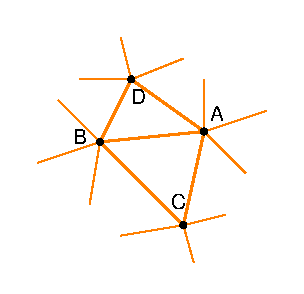
\includegraphics[width=55mm]{malha-tri}
  \caption{A (part of a) triangular mesh}
  \label{\numb section 9.\numb fig 2}
\end{figure}

However, the segments must have reverse.
Consider triangle {\small\tt ABC} for instance.
Its boundary is made of three segments; let's look at {\small\tt AB} for example,
a segment having {\small\tt A} as base (or rather {\small\tt A.reverse()}) and
{\small\tt B} as tip.
Now, a triangle {\small\tt BAD} (no offense intended) also exists as part of
{\small\tt tri\_\,mesh}.
The boundary of {\small\tt BAD} is made of three segments, one of them being {\small\tt BA},
which has {\small\tt B} as base and {\small\tt A} as tip.
{\small\tt AB} and {\small\tt BA} are different {\small\tt \verm{Cell}} objects;
each is the reverse of the other.
They are not two wrappers for the same core, they have different cores.%
\footnote {In contrast, negative meshes share the same core with their positive
counterpart; see paragraph \ref{\numb section 11.\numb parag 4}.}
One of them is considered positive and the other is considered negative.
Which is which depends on which one was built first.
So, all inner segments must have a reverse;
segments on the boundary of {\small\tt tri\_\,mesh} (not visible in figure
\ref{\numb section 9.\numb fig 2}) will probably have no reverse.

For points (vertices), the situation is even more complex.
Segment {\small\tt AB} sees {\small\tt A} as negative because {\small\tt A} is its base
(or rather {\small\tt A.reverse()}),
but other segments like {\small\tt CA} see {\small\tt A} as positive.

Let's look again at iterators described in paragraph \ref{\numb section 9.\numb parag 3}.
We now understand that there is no point to have an iterator over oriented
segments, or over oriented vertices, of {\small\tt tri\_\,mesh}.
That's why iterators over cells of lower dimension always produce positive cells.

We also understand that usually there is no difference between these two iterators :

\begin{Verbatim}[commandchars=\\\{\},formatcom=\small\tt,
   baselinestretch=0.94,framesep=2mm                      ]
   \verm{Mesh}::Iterator \azul{it1} = tri_msh .iterator ( \textcolor{tag}{tag}::over_cells_of_dim, \laranja{2} );
   \verm{Mesh}::Iterator \azul{it2} =
      tri_msh .iterator ( \textcolor{tag}{tag}::over_cells_of_dim, \laranja{2}, \textcolor{tag}{tag}::force_positive );
\end{Verbatim}

\noindent because all triangles composing {\small\tt tri\_\,mesh} should be positive
(use {\small\tt it1}, it is slightly faster).
However, if some of the triangles are negative {\small\tt it1} will behave differently from
{\small\tt it2}.
For instance, if {\small\tt tri\_\,mesh} is the boundary of a polyhedron in $ \mathbb{R}^3 $
and this polyhedron touches other polyhedra (there are shared faces), then it is
quite possible that some of the triangles in {\small\tt tri\_\,mesh} be negative.
If you are aware that your mesh may contain negative cells but
you want to iterate over their positive counterparts, use the {\small\tt \textcolor{tag}{tag}::force\_\,positive}.

We now turn to iterators over one-dimensional meshes, described in paragraph
\ref{\numb section 9.\numb parag 4}.
The two iterators below will probably have different behaviours,
depending on which segments happen to be positive :

\begin{Verbatim}[commandchars=\\\{\},formatcom=\small\tt,
   baselinestretch=0.94,framesep=2mm                      ]
   \verm{Mesh}::Iterator \azul{it3} = ABC .boundary() .iterator ( \textcolor{tag}{tag}::over_segments );
   \verm{Mesh}::Iterator \azul{it4} =
      ABC .boundary() .iterator ( \textcolor{tag}{tag}::over_segments, \textcolor{tag}{tag}::force_positive );
\end{Verbatim}

There is no difference between the two iterators below (both produce positive
points).

\begin{Verbatim}[commandchars=\\\{\},formatcom=\small\tt,
   baselinestretch=0.94,framesep=2mm                      ]
   \verm{Mesh}::Iterator \azul{it5} = ABC .boundary() .iterator ( \textcolor{tag}{tag}::over_vertices, \textcolor{tag}{tag}::backwards );
   \verm{Mesh}::Iterator \azul{it6} = ABC .boundary() .reverse() .iterator ( \textcolor{tag}{tag}::over_vertices );
\end{Verbatim}

However, the two iterators below are quite different.

\begin{Verbatim}[commandchars=\\\{\},formatcom=\small\tt,
   baselinestretch=0.94,framesep=2mm                      ]
   \verm{Mesh}::Iterator \azul{it7} = ABC .boundary() .iterator ( \textcolor{tag}{tag}::over_segments, \textcolor{tag}{tag}::backwards );
   \verm{Mesh}::Iterator \azul{it8} = ABC .boundary() .reverse() .iterator ( \textcolor{tag}{tag}::over_segments );
\end{Verbatim}

Iterator {\small\tt it7} will produce segments {\small\tt AB}, {\small\tt CA}, {\small\tt BC}
(not necessarily beginning at {\small\tt AB}), while {\small\tt it8} will produce their reverses
{\small\tt BA}, {\small\tt AC}, {\small\tt CB} (not necessarily beginning at {\small\tt BA}).

Incidentally, note that a segment, say, {\small\tt BC}, may have no reverse,
for instance if it is on the boundary of {\small\tt tri\_\,mesh}.
However, its reverse {\small\tt CB} will be built on-the-fly (and will stay persistent)
as soon as you use the reverse mesh {\small\tt ABC.boundary().reverse()} in the declaration of
{\small\tt it6} (or {\small\tt it8}, whichever happens first in your code).


          %------------------------%
\section{~~Navigating inside a mesh}\label{\numb section 9.\numb parag 6}
          %------------------------%

Objects in class {\small\tt \verm{Mesh}} have two methods, {\small\tt cell\_\,behind} and
{\small\tt cell\_\,in\_\,front\_\,of},
which provide access to the neighbours of a given cell within that mesh.
Together with methods {\small\tt base} and {\small\tt tip} of class {\small\tt \verm{Cell}}
(mentioned in paragraph \ref{\numb section 1.\numb parag 2}), they allow us to navigate inside
a mesh.

\begin{figure}[ht] \centering
  \psfrag{A}{\small\tt\textcolor{textindraw}{A}}
  \psfrag{B}{\small\tt\textcolor{textindraw}{B}}
  \psfrag{C}{\small\tt\textcolor{textindraw}{C}}
  \psfrag{D}{\small\tt\textcolor{textindraw}{D}}
  \psfrag{hex_1}{\small\tt\textcolor{textindraw}{hex\_\,1}}
  \psfrag{hex_2}{\small\tt\textcolor{textindraw}{hex\_\,2}}
  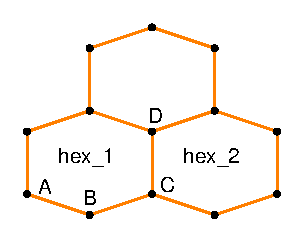
\includegraphics[width=40mm]{malha-hex}
  \caption{A mesh made of hexagons}
  \label{\numb section 9.\numb fig 3}
\end{figure}

Consider the mesh {\small\tt hex\_\,msh} shown in figure \ref{\numb section 9.\numb fig 3},
made of three hexagons.
Pick one of them, at random :

\begin{Verbatim}[commandchars=\\\{\},formatcom=\small\tt,
   baselinestretch=0.94,framesep=2mm                      ]
   \verm{Mesh}::Iterator \azul{it1} = hex_msh .iterator ( \textcolor{tag}{tag}::over_cells_of_dim, \laranja{2} );
   it1 .reset();  assert ( it1 .in_range() );
   \verm{Cell} \azul{hex_1} = *it1;
\end{Verbatim}

Now choose a random segment on the boundary of {\small\tt hex\_\,1} :

\begin{Verbatim}[commandchars=\\\{\},formatcom=\small\tt,
   baselinestretch=0.94,framesep=2mm                      ]
   \verm{Mesh}::Iterator \azul{it2} = hex_1 .boundary() .iterator ( \textcolor{tag}{tag}::over_segments );
   it2 .reset();  assert ( it2 .in_range() );
   \verm{Cell} \azul{AB} = *it2;
\end{Verbatim}

Take its tip :

\begin{Verbatim}[commandchars=\\\{\},formatcom=\small\tt,
   baselinestretch=0.94,framesep=2mm                      ]
   \verm{Cell} \azul{B} = AB .tip();
\end{Verbatim}

Suppose now we want the next segment, within the boundary of {\small\tt hex\_\,1} :

\begin{Verbatim}[commandchars=\\\{\},formatcom=\small\tt,
   baselinestretch=0.94,framesep=2mm                      ]
   \verm{Cell} \azul{BC} = hex_1 .boundary() .cell_in_front_of ( B );
\end{Verbatim}

And now we may continue by taking the tip of {\small\tt BC} and then the segment
following it$\;$:

\begin{Verbatim}[commandchars=\\\{\},formatcom=\small\tt,
   baselinestretch=0.94,framesep=2mm                      ]
   \verm{Cell} \azul{C} = BC .tip();
   \verm{Cell} \azul{CD} = hex_1 .boundary() .cell_in_front_of ( C );
\end{Verbatim}

\noindent an so forth (this is how iterators over vertices and segments of connected
one-dimensional meshes, described in paragraph \ref{\numb section 9.\numb parag 4},
are implemented internally).

Within the mesh {\small\tt hex\_\,msh}, we can navigate towards a neighbour hexagon :

\begin{Verbatim}[commandchars=\\\{\},formatcom=\small\tt,
   baselinestretch=0.94,framesep=2mm                      ]
   \verm{Cell} \azul{hex_2} = hex_msh .cell_in_front_of ( CD );
\end{Verbatim}

Since we have picked {\small\tt hex\_\,1} at random within {\small\tt hex\_\,msh},
as well as {\small\tt AB} within the boundary of {\small\tt hex\_\,1},
there is no guarantee that we actually are in the configuration shown in
Figure \ref{\numb section 9.\numb fig 3}.
That is, {\small\tt CD} may be on the boundary of {\small\tt hex\_\,msh};
there may be no neighbour hexagon {\small\tt hex\_\,2}.
If that is the case, the code above will produce an execution error.
See paragraph \ref{\numb section 9.\numb parag 7} for a way to check whether there is actually
a neighbour cell and thus avoid errors at execution time.

Note that faces point outwards.
For instance, {\small\tt CD} belongs to the boundary of {\small\tt hex\_\,1} and points
outwards, towards {\small\tt hex\_\,2}.
Thus, {\small\tt hex\_\,msh.cell\_\,in\_\,front\_\,of(CD)} produces {\small\tt hex\_\,2}.
On the other hand, {\small\tt hex\_\,msh.cell\_\,behind(CD)} is {\small\tt hex\_\,1}.

Note also that {\small\tt CD} does not belong to the boundary of {\small\tt hex\_\,2}.
If we take {\small\tt hex\_\,2.boundary(). .cell\_\,in\_\,front\_\,of(D)} we will obtain not
{\small\tt CD} but its reverse, a distinct cell which we may call {\small\tt DC}.
We have that {\small\tt hex\_\,msh.cell\_\,in\_\,front\_\,of(DC)} is {\small\tt hex\_\,1} and
{\small\tt hex\_\,msh.cell\_\,behind(DC)} is {\small\tt hex\_\,2}.
Between {\small\tt CD} and {\small\tt DC}, one is positive and the other is negative;
which is which is not very important for the user.


          %------------------------------------%
\section{~~Navigating at the boundary of a mesh}\label{\numb section 9.\numb parag 7}
          %------------------------------------%

Consider the example in paragraph \ref{\numb section 9.\numb parag 6}.
Suppose you try to get a neighbour hexagon which does not exist :

\begin{Verbatim}[commandchars=\\\{\},formatcom=\small\tt,
   baselinestretch=0.94,framesep=2mm                      ]
   \verm{Cell} \azul{no_such_hex} = hex_msh .cell_in_front_of ( AB );
\end{Verbatim}

In {\small\tt DEBUG} mode, you will get an {\small\tt assertion error}.
In {\small\tt NDEBUG} mode, the behaviour is undefined
(often, a {\small\tt segmentation fault} will arise).
The {\small\tt DEBUG} mode is explained in paragraph \ref{\numb section 11.\numb parag 15}.

You may check the existence of the neighbour cell by using a
{\small\tt \textcolor{tag}{tag}::may\_\;not\_\,exist} and then the cell's method {\small\tt exists} :

\begin{Verbatim}[commandchars=\\\{\},formatcom=\small\tt,
   baselinestretch=0.94,framesep=2mm                      ]
   \verm{Cell} \azul{possible_hex} = hex_msh .cell_in_front_of ( AB, \textcolor{tag}{tag}::may_not_exist );
   if ( possible_hex .exists() ) do_something_to ( possible_hex );
   else cout << \verde{"no neighbour !"} << endl;
\end{Verbatim}

\noindent thus avoiding errors at execution time.

Paragraph \ref{\numb section 9.\numb parag 10} gives a complete list of operations which return
an existing cell or build a new one.


          %-----------------------%
\section{~~Iterators around a cell}\label{\numb section 9.\numb parag 8}
          %-----------------------%

Suppose we are looking at a vertex within a mesh and we want to do something to all segments
originating at that vertex, or to all squares touching that vertex, or (depending on the
dimension of the mesh) to all cubes sharing that vertex.

Within this paragraph, in order to simplify the speech, we shall call ``square'' to a generic
cell of dimension 2 (which may be a triangle or a hexagon or some other shape) and
``cube'' to a generic cell of dimension three (which may be a tetrahedron or some other shape).

Another similar situation is when we are looking at a segment in a three-dimensional mesh
and we want to
run over all squares having that segment as edge, or to all cubes having that edge.
These situations require an iterator quite different from the ones described in paragraphs
\ref{\numb section 9.\numb parag 3} and \ref{\numb section 9.\numb parag 4}.
We need an iterator which goes ``around'' a certain cell.

Note that we do not need an iterator to find, in a two-dimensional mesh, the two squares
neighbour to a given segment, or, in a three-dimensional mesh, the two cubes neighbour to
a given square.
We do this by using methods {\small\tt cell\_\,in\_\,front\_\,of} and {\small\tt cell\_\,behind},
as explained in paragraphs \ref{\numb section 9.\numb parag 6} and
\ref{\numb section 9.\numb parag 7}.
Thus, we shall not consider the case when the central cell has co-dimension one, that is,
has dimension equal to the dimension of the mesh minus one.

So, we assume that the co-dimension is two or higher and we distinguish between
the case when the central cell has co-dimension two and the case of co-dimension
three or higher.

To begin with, suppose the central cell has co-dimension three or higher.
The only natural example is a vertex in a three-dimensional mesh (that's co-dimension three).
Less intuitive examples may appear if we play with meshes of (topological) dimension
four or higher.

In code below, we iterate over all segments originating at a given vertex.
The segments will show up in a rahter unpredictable order.

\begin{Verbatim}[commandchars=\\\{\},formatcom=\small\tt,
   baselinestretch=0.94,framesep=2mm                      ]
   \verm{Mesh} \azul{msh} ( \cinza{...} );  \cinza{// a mesh of cubes for instance}
   \verm{Mesh}::Iterator \azul{it} =  \cinza{// P is a positive vertex within msh}
              msh .iterator ( \textcolor{tag}{tag}::over_cells_of_dim, \laranja{1}, \textcolor{tag}{tag}::around, P.reverse() );
   \cinza{// or, equivalently :}
   \cinza{// CellIterator it = msh .iterator ( tag::over_segments, tag::around, P.reverse() )}
   for ( it .reset(); it .in_range(); it++ )
   \{  \verm{Cell} \azul{seg} = *it;  do_something_to ( seg );   \}
\end{Verbatim}

The orientation of the central cell is important in this case.
In the above, we have provided a negative center, {\small\tt P.reverse()};
thus, the iterator will produce segments {\small\tt\azul{seg}} having {\small\tt P} as base
(or rather {\small\tt P.reverse()}) and pointing away from {\small\tt P}.
In contrast, the iterator declared below, having {\small\tt P} as centrall cell,
produces segments pointing towards {\small\tt P}.

\begin{Verbatim}[commandchars=\\\{\},formatcom=\small\tt,
   baselinestretch=0.94,framesep=2mm                      ]
   \verm{Mesh}::Iterator \azul{it} = msh .iterator ( \textcolor{tag}{tag}::over_cells_of_dim, \laranja{1}, \textcolor{tag}{tag}::around, P );
   \cinza{// or, equivalently :}
   \cinza{// CellIterator it = msh .iterator ( tag::over_segments, tag::around, P )}
\end{Verbatim}

In either case, since we are in a three-dimensional mesh, positive or negative segments
{\small\tt seg} may show up.
If you want positive segments, add a {\small\tt\textcolor{tag}{tag}::force\_\,positive} before
{\small\tt\textcolor{tag}{tag}::around} in the declaration of {\small\tt it};
in this case, some of the segments will point towards {\small\tt P},
others will point away from {\small\tt P}.
If you provide a {\small\tt\textcolor{tag}{tag}::force\_\,positive}, it makes no difference
if you give {\small\tt P} or {\small\tt P.reverse()} as central cell in the constructor.

Note that {\small\tt P} may be on the boundary of {\small\tt msh}.
The iterator will produce, of course, only cells belonging to the mesh, including those
on the boundary.

If we want to run over squares or cubes having {\small\tt P} as vertex,
the orientation of the ``center'' {\small\tt P} does not matter.
We can provide a positive vertex {\small\tt P} or a negative one {\small\tt P.reverse()},
this will not change the behaviour of the iterator {\small\tt it} :

\begin{Verbatim}[commandchars=\\\{\},formatcom=\small\tt,
   baselinestretch=0.94,framesep=2mm                      ]
   \verm{Mesh}::Iterator \azul{it} = msh .iterator ( \textcolor{tag}{tag}::over_cells_of_dim, \laranja{2}, \textcolor{tag}{tag}::around, P );
   for ( it .reset(); it .in_range(); it++ )
   \{  \verm{Cell} \azul{cll} = *it;  do_something_to ( cll );   \}
\end{Verbatim}

Such an iterator will produce positive two-dimensional cells.
Again, if {\small\tt P} is the boundary of {\small\tt msh}, the iterator will produce
only cells belonging to the mesh, including those on the boundary.

If we ask for cubes, we will get cells oriented in accordance to the mesh {\small\tt msh}.
Except in exotic examples, these cells will be positive, but if you want to be sure you
can always add the {\small\tt\textcolor{tag}{tag}::force\_\,positive} :

\begin{Verbatim}[commandchars=\\\{\},formatcom=\small\tt,
   baselinestretch=0.94,framesep=2mm                      ]
   \verm{Mesh}::Iterator \azul{it} = msh .iterator ( \textcolor{tag}{tag}::over_cells_of_dim, \laranja{3}, \textcolor{tag}{tag}::force_positive,
                                       \textcolor{tag}{tag}::around, P                                 );
\end{Verbatim}

Consider now the case when the co-dimension is two, that is, when we are centered at a vertex
within a two-dimensional mesh, or at a segment within a three-dimensional mesh.

In this case, the cells around that ``center'' have a natural linear order.
If the ``center'' is at the boundary of {\small\tt msh}, this order is like an
open chain; if the ``center'' is in the interior of {\small\tt msh}, these cells
are organized in a closed loop.
Hence, the constructor of an iterator centered at a cell of co-dimension two accepts
tags like {\small\tt\textcolor{tag}{tag}::backwards} or {\small\tt\textcolor{tag}{tag}::require\_\,order}.
Also, the {\small\tt reset} method accepts the {\small\tt\textcolor{tag}{tag}::start\_\,at} followed
by an argument of type {\small\tt\verm{Cell}}.
Thus, many of the considerations in paragraph \ref{\numb section 9.\numb parag 4}
apply to this type of iterators.

For example, if {\small\tt msh} is a two-dimensional mesh, code below will produce
all squares sharing the vertex {\small\tt P}, linearly ordered.

\begin{Verbatim}[commandchars=\\\{\},formatcom=\small\tt,
   baselinestretch=0.94,framesep=2mm                      ]
   \verm{Mesh}::Iterator \azul{it} = msh .iterator ( \textcolor{tag}{tag}::over_cells_of_dim, \laranja{2}, \textcolor{tag}{tag}::around, P );
\end{Verbatim}

If {\small\tt P} is at the boundary of {\small\tt msh}, the iteration process will begin
with a square adjacent to the boundary and will end when it reaches again the boundary
(which may happen at once if {\small\tt P} is a corner of the mesh).

We can iterate over segments originating at {\small\tt P} (now the orientation of
{\small\tt P} is important) as in:

\begin{Verbatim}[commandchars=\\\{\},formatcom=\small\tt,
   baselinestretch=0.94,framesep=2mm                      ]
   \verm{Mesh}::Iterator \azul{it} = 
               msh .iterator ( \textcolor{tag}{tag}::over_cells_of_dim, \laranja{1}, \textcolor{tag}{tag}::around, P.reverse() );
   \cinza{// or, equivalently :}
   \cinza{// CellIterator it = msh .iterator ( tag::over_segments, tag::around, P.reverse() )}
\end{Verbatim}

If we want to start with a particular square {\small\tt sq}, we specify this by giving
supplementary arguments to the {\small\tt reset} method :

\begin{Verbatim}[commandchars=\\\{\},formatcom=\small\tt,
   baselinestretch=0.94,framesep=2mm                      ]
   \verm{Mesh}::Iterator \azul{it} = msh .iterator ( \textcolor{tag}{tag}::over_cells_of_dim, \laranja{2}, \textcolor{tag}{tag}::around, P );
   for ( it .reset ( \textcolor{tag}{tag}::start_at, sq ); it .in_range(); it++ )
   \{  \verm{Cell} \azul{cll} = *it;  do_something_to ( cll );   \}
\end{Verbatim}

Just like in paragraph \ref{\numb section 9.\numb parag 4}, beware : if {\small\tt P}
is at the boundary of {\small\tt msh}, cells previous to {\small\tt sq} will not
show up.

There are also iterators over vertices around a given vertex.
They simply iterate over the segments originating at that vertex and,
when de-referenced, produce the tip of the current segment.
They provide an ordered sequence of vertices if the surrounding mesh is two-dimensional;
they produce vertices in a rather unpredictable order in a three-dimensional mesh :

\begin{Verbatim}[commandchars=\\\{\},formatcom=\small\tt,
   baselinestretch=0.94,framesep=2mm                      ]
   \verm{Mesh}::Iterator \azul{it} = msh .iterator ( \textcolor{tag}{tag}::over_vertices, \textcolor{tag}{tag}::around, P );
   for ( it .reset(); it .in_range(); it++ )
   \{  \verm{Cell} \azul{Q} = *it;  do_something_to ( Q );   \}
\end{Verbatim}

If you need the cells to show up in a linear order but you are not familiar
with the notion of co-dimension, you can add the {\small\tt\textcolor{tag}{tag}::require\_\,order}
to the {\small\tt\verm{Mesh}::Iterator} constructor;
this way, if in {\small\tt DEBUG} mode, {\maniFEM} will produce a run-time error
if that particular configuration is not compatible with linear ordering
(that is, if the co-dimension of the central cell is not equal to two).
Specifying {\small\tt\textcolor{tag}{tag}::backwards} also informs {\maniFEM} that you want
linear ordering of cells, so you don't have to provide both tags.

As a general rule, de-referencing a {\small\tt\verm{Mesh}::Iterator} does not build a new
cell (it returns a new wrapper to an existing cell).
Iterators around a cell, described in the present paragraph, are a slight exception to this
rule.
When they encounter positive cells having no reverse, they may choose to build the reverse,
negative, cell.
Actually, this may happen even without de-referencing the iterator;
the constructor of the iterator may, in some cases, build a new negative cell
(e.g., the reverse of a face on the boundary of the mesh).
Negative cells are harmless, except that they occupy some space in the computer's memory.
If you really insist that you don't want new cells to appear due to an iterator,
you can provide the {\small\tt\textcolor{tag}{tag}::do\_\,not\_\,build\_\,cells} as an argument
to the constructor, as in

\begin{Verbatim}[commandchars=\\\{\},formatcom=\small\tt,
   baselinestretch=0.94,framesep=2mm                      ]
   \verm{Mesh}::Iterator \azul{it} = msh .iterator
                 ( \textcolor{tag}{tag}::over_segments, \textcolor{tag}{tag}::do_not_build_cells, \textcolor{tag}{tag}::around, P );
\end{Verbatim}


          %--------------------%
\section{~~\cinza{[empty]}}\label{\numb section 9.\numb parag 9}
          %--------------------%


          %--------------------------%
\section{~~Declaring cells and meshes}\label{\numb section 9.\numb parag 10}
          %--------------------------%

As explained in paragraph \ref{\numb section 11.\numb parag 4}, the {\small\tt \verm{Cell}} class
is just a thin wrapper around a {\small\tt \verm{Cell}::Core}, and similarly for {\small\tt \verm{Mesh}}es.

Statements below build a new wrapper for an existing cell or mesh.
No new cell or mesh is created :

\begin{Verbatim}[commandchars=\\\{\},formatcom=\small\tt,
   baselinestretch=0.94,framesep=2mm                      ]
   \verm{Cell} \azul{A} = B;  \cinza{// B is a Cell}
   \verm{Cell} \azul{C} = *it;  \cinza{// 'it' is a CellIterator}
   \verm{Mesh} \azul{msh_copy} = msh;  \cinza{// msh is a Mesh}
   \verm{Mesh} \azul{bd} = cll .boundary();  \cinza{// cll is a Cell of dimension 1 or higher}
\end{Verbatim}

Statements below search for an existing cell.
If the respective cell exists, (a new wrapper for) it is returned.
Otherwise, an {\small\tt assertion error} will occur in {\small\tt DEBUG} mode;
in {\small\tt NDEBUG} mode, the behaviour is undefined (often, a {\small\tt segmentation fault}
will arise).
The {\small\tt DEBUG} mode is explained in paragraph \ref{\numb section 11.\numb parag 15}.

\begin{Verbatim}[commandchars=\\\{\},formatcom=\small\tt,
   baselinestretch=0.94,framesep=2mm                      ]
   \verm{Cell} \azul{A_rev} = A .reverse ( \textcolor{tag}{tag}::surely_exists );  \cinza{//  A is a Cell}
   \cinza{// or, equivalently :}
   \verm{Cell} \azul{A_rev} ( \textcolor{tag}{tag}::reverse_of, A, \textcolor{tag}{tag}::surely_exists );

   \verm{Cell} \azul{tri1} = msh .cell_behind ( CD );  \cinza{//  CD is a Cell, a face within msh}
   \verm{Cell} \azul{tri2} = msh .cell_in_front_of ( CD );
   \cinza{// or, equivalently :}
   \verm{Cell} \azul{tri1} ( \textcolor{tag}{tag}::behind_face, CD, \textcolor{tag}{tag}::within_mesh, msh );
   \verm{Cell} \azul{tri2} ( \textcolor{tag}{tag}::in_front_of_face, CD, \textcolor{tag}{tag}::within_mesh, msh );
   \cinza{// or, equivalently :}
   \verm{Cell} \azul{tri1} = msh .cell_behind ( CD, \textcolor{tag}{tag}::surely_exists );
   \verm{Cell} \azul{tri2} = msh .cell_in_front_of ( CD, \textcolor{tag}{tag}::surely_exists );
   \cinza{// or, equivalently :}
   \verm{Cell} \azul{tri1} ( \textcolor{tag}{tag}::behind_face, CD, \textcolor{tag}{tag}::within_mesh, msh, \textcolor{tag}{tag}::surely_exists );
   \verm{Cell} \azul{tri2} ( \textcolor{tag}{tag}::in_front_of_face, CD,
               \textcolor{tag}{tag}::within_mesh, msh, \textcolor{tag}{tag}::surely_exists );
\end{Verbatim}

Note that reverse meshes exist always (negative meshes are temporary objects built
on-the-fly).

\begin{Verbatim}[commandchars=\\\{\},formatcom=\small\tt,
   baselinestretch=0.94,framesep=2mm                      ]
   \verm{Mesh} \azul{rev_msh} = msh .reverse();  \cinza{// msh is a Mesh}
\end{Verbatim}

Statements below search for an existing cell.
If the respective cell exists, (a new wrapper for) it is returned.
Otherwise, a non-existent cell is returned
(an empty wrapper); the user has the possibility of inquiring the existence
of the returned cell using its method {\small\tt exists}, as illustrated in paragraph
\ref{\numb section 9.\numb parag 7}.

\begin{Verbatim}[commandchars=\\\{\},formatcom=\small\tt,
   baselinestretch=0.94,framesep=2mm                      ]
   \verm{Cell} \azul{A_rev} = A .reverse ( \textcolor{tag}{tag}::may_not_exist );  \cinza{//  A is a Cell}
   \cinza{// or, equivalently :}
   \verm{Cell} \azul{A_rev} ( \textcolor{tag}{tag}::reverse_of, A, \textcolor{tag}{tag}::may_not_exist );
   
   \verm{Cell} \azul{tri1} = msh .cell_behind ( CD, \textcolor{tag}{tag}::may_not_exist );
   \cinza{//  CD is a Cell, a face within msh}
   \verm{Cell} \azul{tri2} = msh .cell_in_front_of ( CD, \textcolor{tag}{tag}::may_not_exist );
   \cinza{// or, equivalently :}
   \verm{Cell} \azul{tri1} ( \textcolor{tag}{tag}::behind_face, CD, \textcolor{tag}{tag}::within_mesh, msh, \textcolor{tag}{tag}::may_not_exist );
   \verm{Cell} \azul{tri2}
      ( \textcolor{tag}{tag}::in_front_of_face, CD, \textcolor{tag}{tag}::within_mesh, msh, \textcolor{tag}{tag}::may_not_exist );
\end{Verbatim}

Statements below return a previously built cell, if it exists.
If that object does not exist, it is built on-the-fly.

\begin{Verbatim}[commandchars=\\\{\},formatcom=\small\tt,
   baselinestretch=0.94,framesep=2mm                      ]
   \verm{Cell} \azul{A_rev} = A .reverse();  \cinza{// A is some Cell}
   \cinza{// or, equivalentely :}
   \verm{Cell} \azul{A_rev} ( \textcolor{tag}{tag}::reverse_of, A );
   \cinza{// or, equivalentely :}
   \verm{Cell} \azul{A_rev} = A .reverse ( \textcolor{tag}{tag}::build_if_not_exists );
   \cinza{// or, equivalentely :}
   \verm{Cell} \azul{A_rev} ( \textcolor{tag}{tag}::reverse_of, A, \textcolor{tag}{tag}::build_if_not_exists );
\end{Verbatim}

De-referencing a {\small\tt\verm{Mesh}::Iterator} returns (a new wrapper for) an existing cell;
a slight exception to this rule is described in paragraph \ref{\numb section 9.\numb parag 8}.

Statements below return a wrapper for a brand new cell or mesh :

\begin{Verbatim}[commandchars=\\\{\},formatcom=\small\tt,
   baselinestretch=0.94,framesep=2mm                      ]
   \verm{Cell} \azul{A} ( \textcolor{tag}{tag}::vertex );
   \verm{Mesh} \azul{AB} ( \textcolor{tag}{tag}::segment, A .reverse(), B, \textcolor{tag}{tag}::divided_in, 15 );
   \cinza{// B is another vertex Cell}
   \verm{Mesh} \azul{ABC} ( \textcolor{tag}{tag}::triangle, AB, BC, CA );
   \cinza{//  BC and CA are segment Meshes, each having 15 segments Cells}
   \cinza{// ... and many other shapes ...}
\end{Verbatim}

% Paragraph \ref{\numb section 11.\numb parag 8} explains similar operations
% on {\small\tt \verm{Cell}::Core}s.


